% !TEX program = xelatex
% Zeva v2: preserve the selected draft's illustrations throughout the page.
% Every \art call is a viewport into the unmodified 1254 x 1254 imagegen draft.
% This is a mixed raster/vector PDF, not an all-vector illustration.
% Formulae and computation flow: user Scholaread PDF, Fig. 2, Eq. 3--8,
% Algorithm 1, III-C--F, IV-A.1. See ../tmp/drawpaper-spec.md.
\documentclass[tikz,border=2mm]{standalone}
\usepackage{fontspec,xeCJK,amsmath,amssymb,lmodern,graphicx}
\setsansfont{Arial}
\setCJKmainfont[Path=/System/Library/Fonts/,BoldFont={STHeiti Medium.ttc}]{STHeiti Light.ttc}
\setCJKsansfont[Path=/System/Library/Fonts/,BoldFont={STHeiti Medium.ttc}]{STHeiti Light.ttc}
\renewcommand{\familydefault}{\sfdefault}
\usetikzlibrary{arrows.meta,calc,backgrounds,shadings}
\definecolor{ink}{HTML}{10274B}
\definecolor{muted}{HTML}{426184}
\definecolor{blue}{HTML}{398CC5}
\definecolor{bluebg}{HTML}{E9F8FF}
\definecolor{bluefill}{HTML}{C7EAFB}
\definecolor{purple}{HTML}{8743C5}
\definecolor{purplebg}{HTML}{F1E9FC}
\definecolor{purplefill}{HTML}{DBC3F3}
\definecolor{orange}{HTML}{EB772D}
\definecolor{orangebg}{HTML}{FFF3E2}
\definecolor{teal}{HTML}{49A996}
\definecolor{red}{HTML}{DC593E}
\definecolor{edge}{HTML}{B7C8D5}
\definecolor{cream}{HTML}{F7F5EF}
\tikzset{t/.style={text=ink,font=\fontsize{13.5}{16}\selectfont,align=center,inner sep=0,outer sep=0},
  sm/.style={t,font=\fontsize{12}{14.5}\selectfont},
  hd/.style={t,font=\bfseries\fontsize{18}{21}\selectfont},
  card/.style={rounded corners=5pt,line width=.65pt},
  a/.style={-{Stealth[length=2.4mm,width=1.7mm]},draw=ink,line width=1.1pt,rounded corners=2pt},
  ba/.style={a,draw=blue},pa/.style={a,draw=purple,line width=1.5pt},
  oa/.style={a,draw=orange},ra/.style={a,draw=red,line width=1.6pt}}
\newcommand{\txt}[4]{\node[t,text width=#3*.3mm]at(#1,#2){#4};}
\newcommand{\sm}[4]{\node[sm,text width=#3*.3mm]at(#1,#2){#4};}
\newcommand{\head}[4]{\node[hd,text width=#3*.3mm]at(#1,#2){#4};}
\newcommand{\maths}[4]{\node[t,font=\fontsize{#3}{#3}\selectfont]at(#1,#2){\(\displaystyle #4\)};}
\newcommand{\boxc}[7]{\draw[card,draw=#5,fill=#6](#1,#2)rectangle++(#3,#4);\txt{#1+#3/2}{#2+#4/2}{#3-8}{#7}}
% Graphicx crops the original bitmap at PDF assembly time. No asset editing.
\newcommand{\art}[7]{\begingroup
  \pgfmathsetmacro{\btrim}{1254-#2-#4}
  \pgfmathsetmacro{\rtrim}{1254-#1-#3}
  \pgfmathsetlengthmacro{\awidth}{#7*.3mm}
  \node[anchor=north west,inner sep=0,outer sep=0]at(#5,#6){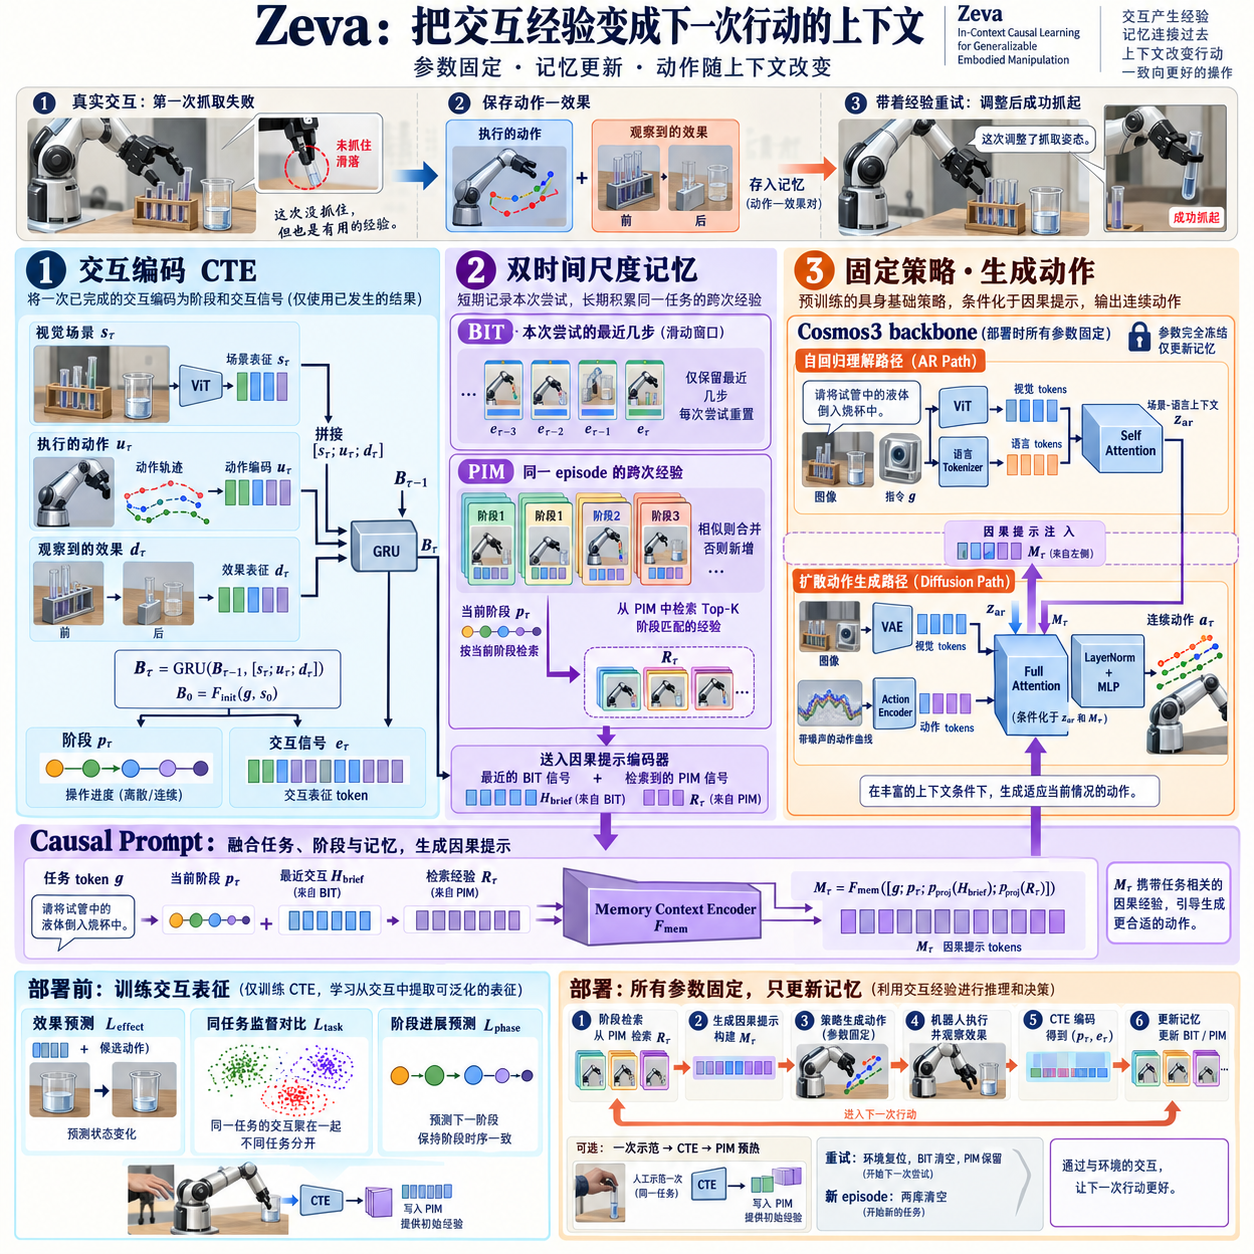
\includegraphics[trim=#1bp \btrim bp \rtrim bp #2bp,clip,width=\awidth]{zeva-illustrated-v1-imagegen-draft.png}};
\endgroup}
\newcommand{\tokens}[5]{\foreach \i in {0,...,#3}{\shade[left color=#5!30,right color=#5!65,draw=#5,line width=.5pt]({#1+\i*(#4+3)},#2)rectangle++(#4,20);}}
\newcommand{\phase}[3]{\draw[ink!60,line width=.7pt](#1,#2)--++(#3*4,0);\foreach \i/\c in {0/orange,1/teal,2/blue,3/purple,4/purple}{\shade[ball color=\c!60,draw=\c,line width=.6pt](#1+\i*#3,#2)circle(6);}}
\newcommand{\prism}[6]{\shade[left color=#5!35,right color=#5!60,draw=#5,line width=.85pt](#1+13,#2+10)--(#1+#3,#2+10)--(#1+#3,#2+#4)--(#1+13,#2+#4)--cycle;\shade[top color=#5!15,bottom color=#5!35,draw=#5,line width=.85pt](#1,#2)--(#1+#3-13,#2)--(#1+#3,#2+10)--(#1+13,#2+10)--cycle;\shade[left color=#5!60,right color=#5!35,draw=#5,line width=.85pt](#1,#2)--(#1+13,#2+10)--(#1+13,#2+#4)--(#1,#2+#4-10)--cycle;\txt{#1+#3/2+6}{#2+#4/2+5}{#3-18}{#6}}

\begin{document}
\begin{tikzpicture}[x=.3mm,y=-.3mm]
\path[use as bounding box](0,0)rectangle(1254,1390);
\fill[white](0,0)rectangle(1254,1390);
\node[t,font=\bfseries\fontsize{29}{32}\selectfont]at(627,28){Zeva：把交互经验变成下一次行动的上下文};
\node[t,font=\fontsize{17}{20}\selectfont]at(627,65){参数固定\quad ·\quad 记忆更新\quad ·\quad 动作随上下文改变};

% Top narrative: retain the realistic arm, close-up, trajectories and outcomes.
\draw[card,draw=edge,fill=cream](16,87)rectangle(1239,241);
\head{208}{103}{368}{1\quad 真实交互：抓取失手}
\head{605}{103}{390}{2\quad 保存动作—效果}
\head{1018}{103}{407}{3\quad 带着经验调整动作}
\art{28}{119}{225}{113}{27}{119}{225}
\art{258}{116}{124}{78}{257}{116}{124}
\sm{320}{216}{126}{这次没抓住，\\也是有用的经验。}
\draw[ba,line width=4pt](394,171)--(429,171);
\boxc{446}{120}{125}{113}{blue}{bluebg}{}
\txt{509}{134}{121}{执行的动作}
\art{450}{148}{116}{80}{450}{148}{116}
\txt{582}{176}{15}{+}
\boxc{594}{120}{146}{113}{orange}{orangebg}{}
\txt{667}{135}{143}{观测到的效果}
\art{598}{150}{132}{60}{599}{153}{132}
\sm{628}{220}{50}{前}
\sm{704}{220}{50}{后}
\sm{785}{198}{89}{存入记忆}
\draw[oa,line width=4pt](750,171)--(825,171);
\art{841}{119}{257}{110}{840}{119}{257}
\art{1108}{108}{116}{123}{1108}{119}{107}

% Original three-column rhythm, including vertical illustrated CTE inputs.
\draw[card,draw=blue!55,fill=bluebg](16,249)rectangle(439,818);
\draw[card,draw=purple!60,fill=purplebg](449,249)rectangle(777,818);
\draw[card,draw=orange!65,fill=orangebg](787,249)rectangle(1239,818);
\head{218}{272}{391}{1\quad 交互编码 CTE}
\head{613}{272}{316}{2\quad 双时间尺度记忆}
\head{1013}{272}{438}{3\quad 固定策略 · 生成动作}
\sm{227}{300}{404}{一次已完成的交互 → 阶段与交互信号}
\sm{613}{300}{313}{近期交互 + 同一 episode 内跨次经验}
\sm{1013}{300}{433}{条件化因果提示，生成连续动作}

% CTE visuals, extracted from the selected draft rather than icon substitutes.
\boxc{28}{322}{271}{105}{blue!50}{bluebg}{}
\txt{98}{335}{132}{视觉场景}
\maths{232}{335}{13.5}{s_\tau}
\art{36}{346}{133}{78}{35}{345}{133}
\prism{178}{365}{45}{43}{blue}{ViT}
\draw[a](169,386)--(178,386);
\tokens{237}{375}{3}{10}{blue}
\sm{258}{361}{72}{视觉特征}
\boxc{28}{434}{271}{105}{blue!50}{bluebg}{}
\txt{96}{448}{132}{执行的动作}
\maths{232}{448}{13.5}{u_\tau}
\art{35}{456}{78}{71}{35}{460}{78}
\art{123}{480}{82}{43}{120}{481}{82}
\sm{162}{466}{86}{动作轨迹}
\draw[a](204,502)--(219,502);
\tokens{225}{491}{4}{10}{teal}
\boxc{28}{546}{271}{105}{blue!50}{bluebg}{}
\txt{104}{560}{150}{观测到的效果}
\maths{248}{560}{13.5}{d_\tau}
\art{33}{570}{68}{55}{34}{578}{68}
\art{121}{572}{68}{53}{121}{578}{68}
\draw[a](105,603)--(117,603);
\draw[a](195,603)--(218,603);
\tokens{225}{594}{4}{10}{purple}
\sm{67}{641}{56}{前}
\sm{157}{641}{56}{后}
\sm{262}{581}{74}{效果特征}
\draw[a](300,386)--(329,386)--(329,539)--(350,539);
\draw[a](300,502)--(319,502)--(319,550)--(350,550);
\draw[a](300,603)--(337,603)--(337,562)--(350,562);
\txt{380}{443}{92}{拼接输入}
\maths{380}{469}{13}{[s_\tau;u_\tau;d_\tau]}
\art{351}{522}{65}{51}{351}{522}{65}
\maths{399}{493}{14}{B_{\tau-1}}
\draw[a](399,506)--(399,519);
\draw[a](417,549)--(429,549)--(429,683)--(326,683);
\maths{419}{580}{14}{B_\tau}
\boxc{40}{663}{372}{49}{blue}{white}{}
\maths{219}{677}{13}{B_\tau=\operatorname{GRU}(B_{\tau-1},[s_\tau;u_\tau;d_\tau])}
\maths{220}{701}{13}{B_0=F_{\mathrm{init}}(g,s_0)\qquad(3)}
\draw[a](220,713)--(220,723)--(132,723)--(132,730);
\draw[a](220,723)--(328,723)--(328,730);
\boxc{28}{733}{188}{75}{blue!50}{bluebg}{}
\boxc{228}{733}{198}{75}{blue!50}{bluebg}{}
\txt{83}{747}{97}{阶段}
\maths{151}{747}{14}{p_\tau}
\phase{54}{769}{34}
\sm{121}{796}{171}{任务进展}
\txt{304}{747}{135}{交互信号}
\maths{392}{747}{14}{e_\tau}
\tokens{244}{761}{9}{11}{purple}
\sm{325}{797}{184}{动作造成的动态效果}
\draw[pa](427,773)--(443,773)--(443,385)--(460,385);
\draw[pa](443,511)--(460,511);

% BIT/PIM keep the full miniature robot cards and their original shading.
\boxc{458}{318}{310}{131}{purple!70}{purplebg}{}
\head{608}{333}{293}{BIT · 本次尝试的最近几步}
\art{478}{356}{189}{66}{480}{357}{187}
\sm{715}{393}{88}{滑动窗口\\保留近期交互}
\maths{501}{435}{12}{e_{\tau-3}}
\maths{549}{435}{12}{e_{\tau-2}}
\maths{596}{435}{12}{e_{\tau-1}}
\maths{644}{435}{12}{e_\tau}
\boxc{458}{459}{310}{278}{purple!70}{purplebg}{}
\node[t,font=\bfseries\fontsize{15}{18}\selectfont]at(613,477){PIM · 同一 episode 的跨次经验};
\art{464}{491}{227}{96}{464}{493}{227}
\node[sm,font=\fontsize{11}{14}\selectfont,text width=67*.3mm]at(727,545){相似则合并\\否则新增};
\txt{527}{612}{130}{当前阶段}
\maths{526}{637}{13.5}{p_\tau}
\phase{476}{659}{18}
\sm{516}{687}{111}{按阶段检索}
\sm{672}{613}{171}{从 PIM 检索\\阶段匹配的交互信号}
\draw[pa](558,659)--(572,659)--(572,697)--(590,697);
\art{585}{648}{176}{71}{585}{653}{176}
\boxc{458}{748}{310}{59}{purple!65}{purplebg}{}
\txt{613}{763}{294}{近期 BIT 信号 + 检索到的 PIM 信号}
\tokens{473}{779}{6}{10}{blue}
\tokens{648}{779}{6}{10}{purple}

% Two-path foundation model. Block faces retain depth, miniature cameras,
% lab scenes, noisy curves, token strips, and action-output robot art.
\head{981}{333}{368}{Cosmos3 backbone}
\art{1127}{320}{25}{34}{1198}{318}{25}
\boxc{797}{350}{431}{195}{orange}{orangebg}{}
\node[t,anchor=west,font=\bfseries\fontsize{14.5}{17}\selectfont,text=orange]at(806,365){自回归理解路径 · AR Path};
\art{803}{427}{120}{60}{804}{389}{120}
\boxc{806}{462}{119}{43}{edge}{white}{将试管中的液体\\倒入烧杯中。}
\prism{940}{390}{47}{42}{blue}{ViT}
\art{938}{433}{51}{54}{939}{443}{51}
\draw[a](925,413)--(938,413);
\draw[a](925,480)--(932,480)--(932,469)--(938,469);
\tokens{1005}{401}{4}{9}{blue}
\tokens{1005}{456}{4}{9}{orange}
\draw[a](989,412)--(1002,412);
\draw[a](989,467)--(1002,467);
\sm{1032}{390}{83}{视觉 tokens}
\sm{1031}{445}{83}{语言 tokens}
\prism{1079}{405}{96}{72}{blue}{Self\\Attention}
\draw[a](1067,412)--(1074,412)--(1074,437)--(1080,437);
\draw[a](1067,466)--(1074,466)--(1074,449)--(1080,449);
\boxc{1055}{488}{151}{26}{blue!60}{white}{LayerNorm + MLP}
\draw[a](1122,475)--(1122,487);
\sm{865}{530}{129}{图像与任务指令}
\sm{1110}{533}{204}{多模态上下文}

\boxc{797}{563}{431}{238}{orange}{orangebg}{}
\node[t,anchor=west,font=\bfseries\fontsize{14.5}{17}\selectfont,text=orange]at(806,578){扩散动作生成路径 · Diffusion Path};
\art{802}{601}{62}{55}{803}{604}{62}
\art{800}{682}{63}{47}{802}{683}{63}
\prism{873}{606}{41}{48}{blue}{VAE}
\art{872}{678}{45}{55}{871}{678}{47}
\draw[a](866,632)--(871,632);
\draw[a](866,707)--(871,707);
\tokens{922}{617}{3}{9}{blue}
\tokens{922}{692}{3}{9}{purple}
\sm{831}{671}{66}{图像}
\sm{843}{746}{83}{带噪动作}
\art{992}{635}{79}{101}{992}{635}{79}
\shade[left color=blue!25,right color=blue!45](1008,709)rectangle(1070,731);
\sm{1040}{722}{62}{条件融合}
\draw[a](970,628)--(982,628)--(982,665)--(991,665);
\draw[a](970,703)--(985,703)--(985,706)--(991,706);
\art{1073}{638}{75}{70}{1078}{639}{72}
\draw[a](1073,679)--(1079,679);
\art{1148}{632}{77}{122}{1148}{631}{77}
\draw[a](1147,673)--(1154,673);
\sm{1182}{617}{83}{连续动作}
\maths{1182}{774}{15}{a_t}
\sm{918}{780}{210}{上下文改变后续动作}
\maths{1027}{612}{13}{z_{\mathrm{AR}}}
\maths{1091}{755}{14}{\mathcal M_\tau}
\draw[ba,line width=1.4pt](1208,501)--(1220,501)--(1220,595)--(979,595)--(979,650)--(992,650);

% Causal Prompt is a visual focal point, using the exact selected encoder art.
\draw[card,draw=purple!60,fill=purplebg](16,827)rectangle(1239,970);
\head{156}{845}{263}{Causal Prompt}
\txt{769}{846}{451}{融合任务、阶段与记忆，生成因果提示}
\draw[pa,line width=2.4pt](608,810)--(608,822)--(398,822)--(398,864);
\boxc{27}{866}{518}{74}{purple!45}{white}{}
\sm{84}{879}{108}{任务条件}
\sm{209}{879}{103}{当前阶段}
\sm{333}{879}{116}{近期交互}
\sm{473}{879}{121}{检索经验}
\boxc{34}{893}{107}{39}{edge}{white}{将试管中的液体\\倒入烧杯中。}
\phase{171}{913}{16}
\tokens{279}{902}{5}{12}{blue}
\tokens{421}{902}{5}{12}{purple}
\draw[pa](544,912)--(559,912);
\art{562}{869}{201}{78}{562}{866}{201}
\draw[pa](764,909)--(807,909);
\boxc{812}{866}{293}{75}{purple!55}{white}{}
\sm{956}{880}{275}{任务相关的因果上下文}
\tokens{832}{903}{11}{16}{purple}
\maths{1149}{877}{15}{\mathcal M_\tau}
\sm{1170}{915}{111}{引导生成\\后续动作}
\draw[pa,line width=3.1pt](1034,865)--(1034,738);
\node[t,font=\fontsize{14}{17}\selectfont]at(637,955){\(\displaystyle\mathcal M_\tau=F_{\mathrm{mem}}\!\left([g;\,p_\tau;\,P_{\mathrm{proj}}(\mathcal H_\tau^{\mathrm{brief}});\,P_{\mathrm{proj}}(\mathcal R_\tau)]\right)\)\quad(8)};

% Training: retain beakers, clusters, stage progression and demonstration art.
\boxc{16}{979}{538}{259}{blue!65}{bluebg}{}
\head{275}{997}{511}{部署前：训练交互表征}
\boxc{27}{1019}{154}{140}{blue!45}{white}{}
\boxc{190}{1019}{178}{140}{blue!45}{white}{}
\boxc{379}{1019}{164}{140}{blue!45}{white}{}
\txt{104}{1034}{148}{效果预测}
\maths{104}{1057}{12.5}{\mathcal L_{\mathrm{effect}}}
\art{31}{1064}{137}{62}{31}{1068}{137}
\node[sm,font=\fontsize{10.5}{12}\selectfont,text width=145*.3mm]at(104,1145){交互信号 + 候选动作\\预测状态变化};
\txt{279}{1034}{169}{同任务监督对比}
\maths{279}{1057}{12.5}{\mathcal L_{\mathrm{task}}}
\art{209}{1050}{143}{65}{208}{1070}{143}
\sm{279}{1145}{169}{同任务交互表征聚拢}
\txt{461}{1034}{152}{阶段进展}
\maths{461}{1057}{12.5}{\mathcal L_{\mathrm{phase}}}
\art{391}{1066}{143}{23}{391}{1087}{143}
\sm{461}{1137}{150}{约束交互表征\\与阶段推进一致}
\art{128}{1167}{159}{66}{30}{1166}{159}
\boxc{207}{1181}{53}{31}{blue}{white}{CTE}
\draw[ba](191,1197)--(205,1197);
\sm{401}{1186}{269}{交互轨迹 → 三项目标 → 更新 CTE}
\draw[draw=red,dashed,line width=.9pt](104,1159)--(104,1163)--(461,1163)--(461,1159);
\draw[draw=red,dashed,line width=.9pt](279,1159)--(279,1163);
\draw[a,draw=red,dashed](233,1163)--(233,1180);
\sm{406}{1225}{254}{训练时更新 · 部署时固定}

% Deployment: all six stages retain visual content rather than bare boxes.
\boxc{565}{979}{674}{259}{orange!65}{orangebg}{}
\head{900}{997}{655}{部署：参数固定，只更新状态与记忆}
\foreach \x in {576,688,799,910,1021,1132}{\draw[card,draw=edge!65,fill=white](\x,1019)rectangle++(99,96);}
\sm{625}{1034}{94}{1\quad 阶段检索}
\sm{737}{1034}{94}{2\quad 构建提示}
\sm{848}{1034}{94}{3\quad 策略出动作}
\sm{959}{1034}{94}{4\quad 执行并观测}
\sm{1070}{1034}{94}{5\quad CTE 编码}
\sm{1181}{1034}{94}{6\quad 更新记忆}
\art{577}{1049}{91}{45}{580}{1055}{90}
\art{694}{1054}{80}{27}{696}{1064}{82}
\art{796}{1046}{91}{58}{803}{1050}{91}
\art{908}{1046}{92}{58}{914}{1050}{92}
\art{1023}{1048}{88}{42}{1027}{1058}{88}
\art{1128}{1047}{99}{48}{1136}{1055}{91}
\foreach \x in {677,789,900,1011,1122}{\draw[oa,line width=1.6pt](\x,1076)--++(9,0);}
\draw[ra,line width=2pt](1180,1117)--(1180,1135)--(625,1135)--(625,1117);
\node[sm,text=red,fill=orangebg,inner sep=2pt]at(901,1135){将真实效果写入记忆，再进入下一步};
\boxc{576}{1153}{251}{75}{edge}{cream}{}
\sm{701}{1167}{241}{可选：一次示范 → CTE → PIM 预热}
\art{577}{1167}{45}{57}{580}{1176}{40}
\art{691}{1170}{113}{48}{670}{1180}{95}
\sm{644}{1200}{47}{人类\\引导}
\boxc{837}{1153}{391}{75}{edge}{cream}{}
\sm{1031}{1173}{374}{重试：环境复位，BIT 与循环状态重置}
\sm{1031}{1197}{374}{同一 episode 保留 PIM；新 episode 两库清空}
\sm{1031}{1220}{374}{先执行，再观测和写记忆\quad ·\quad Algorithm 1}

% Compact precision supplement: preserve the illustrated layout above.
\draw[card,draw=purple!55,fill=purplebg!60](16,1248)rectangle(1239,1382);
\txt{210}{1266}{371}{BIT · 近期窗口\quad(4)}
\txt{824}{1266}{764}{PIM · 按当前阶段检索\quad(7)}
\maths{210}{1296}{14}{\mathcal H_\tau^{\mathrm{brief}}=\{e_j\}_{j=\tau-K_{\mathrm{brief}}}^{\tau}}
\maths{820}{1296}{14}{\mathcal R_\tau=\{e_k\mid(p_k,e_k)\in\mathcal H_\tau^{\mathrm{pim}},\;\operatorname{top}\!\text{-}\!K\;\operatorname{sim}(p_\tau,p_k)\}}
\draw[purple!25](28,1319)--(1227,1319);
\txt{128}{1340}{195}{PIM · 合并评分}
\maths{734}{1340}{14.5}{S_{\mathrm{merge}}(\xi_\tau,\xi_j)=\beta_p\operatorname{sim}(p_\tau,p_j)+\beta_e\operatorname{sim}(e_\tau,e_j)\qquad(5)}
\sm{630}{1367}{1192}{最高分超过阈值：Merge 并替换对应记录；否则新增。\quad 合并看阶段与效果，检索只看阶段。\quad(6)}
\end{tikzpicture}
\end{document}
